\begin{problem}[03]
自由落体问题有哪几种提法? 各有哪些基本量和导出量?
\end{problem}
% --------------------------------------------------------------------

\begin{solution}
\begin{minipage}[c]{0.8\linewidth}
自由落体问题涉及的物理量有高度$h$, 重力加速度$g$, 下落时间$t$. 可取任意两个量为基本量, 另一量为导出量, 因此自由落体问题有以下三种提法:
\begin{itemize}
\item 已知$h$, $g$, 求$t$. 以$h$, $g$为基本量, $t$为导出量: $t = f(h,g)$.
\item 已知$g$, $t$, 求$h$. 以$g$, $t$为基本量, $h$为导出量: $h = f(g,t)$.
\item 已知$h$, $t$, 求$t$. 以$h$, $t$为基本量, $g$为导出量: $g = f(h,t)$.
\end{itemize}
\end{minipage}
\begin{minipage}[c]{0.2\linewidth}
\begin{center}
\usetikzlibrary{%
    decorations.pathreplacing,%
    decorations.pathmorphing,arrows
}
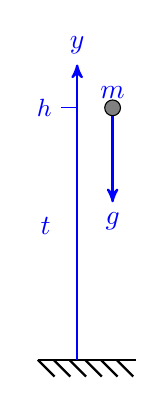
\begin{tikzpicture}[ media/.style={font={\footnotesize\sffamily}},
    wave/.style={
        decorate,decoration={snake,post length=1.4mm,amplitude=2mm,
        segment length=2mm},thick},
    interface/.style={
        postaction={draw,decorate,decoration={border,angle=-45,
                    amplitude=0.3cm,segment length=2mm}}}]
\draw[thick,interface](-0.5,0)--(0.75,0);
\draw[ ->,>=stealth',thick,blue](0,0) -- (0,3.75) node[above]{$y$};

\draw[blue] (0,3.2)--(-.2,3.2) node[left,blue]{\small $h$};
\draw [blue,->,>=stealth',thick] (0.45,3.2) -- (0.45, 2) node [below]{$g$};
\draw [fill=gray](0.45,3.2) circle(0.1) node [above,blue]{$m$};
\node[blue] at (-0.4, 1.7) {$t$};
\end{tikzpicture}
\end{center}
\end{minipage}
\end{solution}
